% In your document preamble: \usepackage{booktabs}, \usepackage{hyperref}, \usepackage{longtable}, \usepackage{caption}
\scriptsize
\setlength{\tabcolsep}{3pt}
\begin{longtable}{llllrr@{\hspace{0.8cm}}llllrr}
\captionsetup{labelformat=empty}
\caption{\textbf{SI Table S13. Data for Ubiquitin Domain Receptors}}
\label{tab:st13} \\
\toprule
apo\_pdb & holo\_pdb & apo\_bmrb & holo\_bmrb & F1 & MCC & apo\_pdb & holo\_pdb & apo\_bmrb & holo\_bmrb & F1 & MCC \\
\midrule
\endfirsthead
\caption[]{(continued)} \\
\toprule
apo\_pdb & holo\_pdb & apo\_bmrb & holo\_bmrb & F1 & MCC & apo\_pdb & holo\_pdb & apo\_bmrb & holo\_bmrb & F1 & MCC \\
\midrule
\endhead
\bottomrule
\endfoot
\bottomrule
\endlastfoot
 & \href{https://www.rcsb.org/structure/2MUR}{2MUR} & \href{https://bmrb.io/data_library/summary/index.php?bmrbId=17769}{17769} & \href{https://bmrb.io/data_library/summary/index.php?bmrbId=25230}{25230} & 0.40 & 0.32 &  & \href{https://www.rcsb.org/structure/2MUR}{2MUR} & \href{https://bmrb.io/data_library/summary/index.php?bmrbId=25229}{25229} & \href{https://bmrb.io/data_library/summary/index.php?bmrbId=25230}{25230} & 0.57 & 0.26 \\
 & \href{https://www.rcsb.org/structure/5VF0}{5VF0} & \href{https://bmrb.io/data_library/summary/index.php?bmrbId=17769}{17769} & \href{https://bmrb.io/data_library/summary/index.php?bmrbId=30276}{30276} & 0.31 & 0.27 &  &  &  &  &  &  \\
\end{longtable}

\begin{figure}[htbp]
\centering
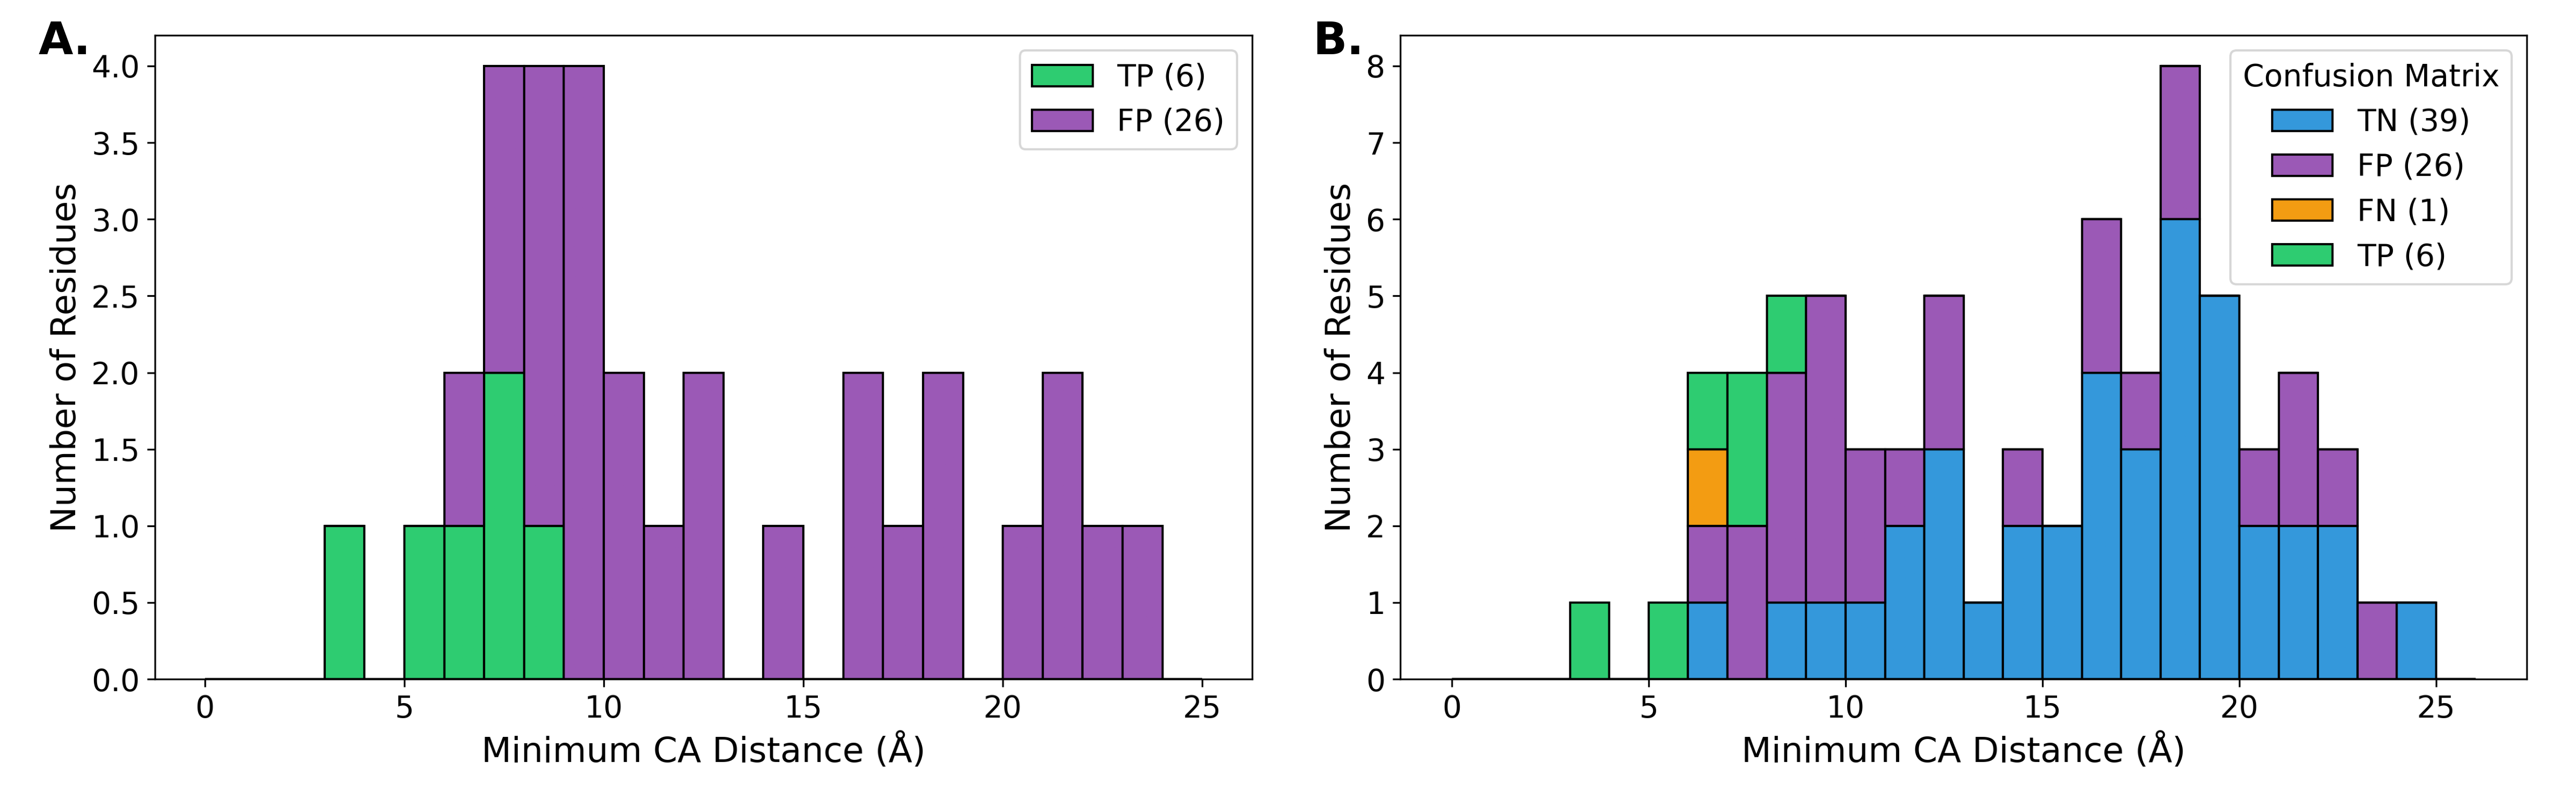
\includegraphics[width=\linewidth]{SF12_ubiquitin.png}
\captionsetup{labelformat=empty}
\caption{\textbf{SI Fig. S12. Confusion Matrix Histograms for Ubiquitin Domain Receptors}}
\label{fig:sf12_ubiquitin}
\end{figure}
